%%%%%%%%%%%%%%%%%%%%%%%%%%%%%%%%%%%%%%%%%%%%%%%%%%%%%%%%%%%%%%%%%%%%%%%%%%%%%%%%%%%%%%%%%
% Section 4: Xilinx Devices
%	This section contains a description of the following:
%	- Vivado FPGA devices (with terminology)
%	- Device data structures in RapidSmith, 
%	- Device files and XDLRC files  
%	- Step-by-step guide on how to intall new devices  
%%%%%%%%%%%%%%%%%%%%%%%%%%%%%%%%%%%%%%%%%%%%%%%%%%%%%%%%%%%%%%%%%%%%%%%%%%%%%%%%%%%%%%%%%
\newpage
\section{Devices}

\subsection{Xilinx FPGA Architecture Overview} \label{fpgaArch}
This section is intended to give a brief introduction to Xilinx FPGA
architecture and terminology. The terminology introduced here is consistent
with the terminolgy used in the Vivado Design Suite. If you are already familiar
with Xilinx FPGA devices, then you can skip to \autoref{devicesRS2}. 
As you read through this section, it may be helpful to open a sample device in Vivado's
Device Browser. To do this, open a new command prompt and run Vivado in Tcl mode
(``vivado -mode tcl''). Then, run the following commands in the Vivado prompt:

\begin{verbatim}
Vivado% link_design -part xc7a100tcsg324-3 -quiet
Vivado% start_gui
\end{verbatim}

\noindent
After these commands are run, a GUI view should pop up showing the components
of an Artix7 FPGA part. Use this to explore the Xilinx device architecture if
needed.

\subsubsection{Tiles}
Conceptually, a Xilinx FPGA can be thought of as a two dimensional
array of \cls{Tile}s. A \cls{Tile} is a template section within a FPGA that
performs a specific function (i.e. implementing logic equations). Templates are
then duplicated across the device (all copies are identical) and different
\cls{Tile} types are wired together. As an example, \autoref{fig:tileExample}
displays three types of template \cls{Tile}s in an Artix7 part.

\begin{figure}[H]
 \centering
 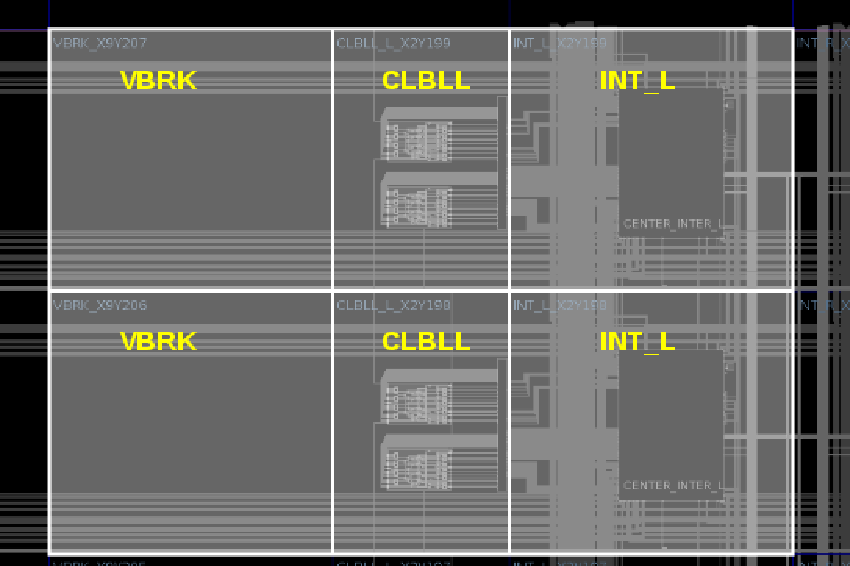
\includegraphics[width=0.7\columnwidth]{tiles}
 \caption{Highlighted example \cls{Tile}s in an Artix7 FPGA.}
 \label{fig:tileExample}
\end{figure}

\noindent
The two \pgm{VBRK} \cls{Tile}s on the left are used for intermediate wiring.
The two \pgm{INT\_L} \cls{Tile}s on the right are switchbox \cls{Tile}s.
These are reconfigurable routing \cls{Tile}s that allow a single wire to go
multiple different locations within the FPGA. The two \pgm{CLBLL} \cls{Tile}s
in the middle are used to implement combinational and sequential digital logic.
They are the basic building blocks of Xilinx FPGAs. Other \cls{Tile} types
include DSP, BRAM, and IOB.
 
\subsubsection{Primitive Sites}

\begin{figure}[b!]
\centering
   \begin{subfigure}[b!]{0.65\textwidth}
   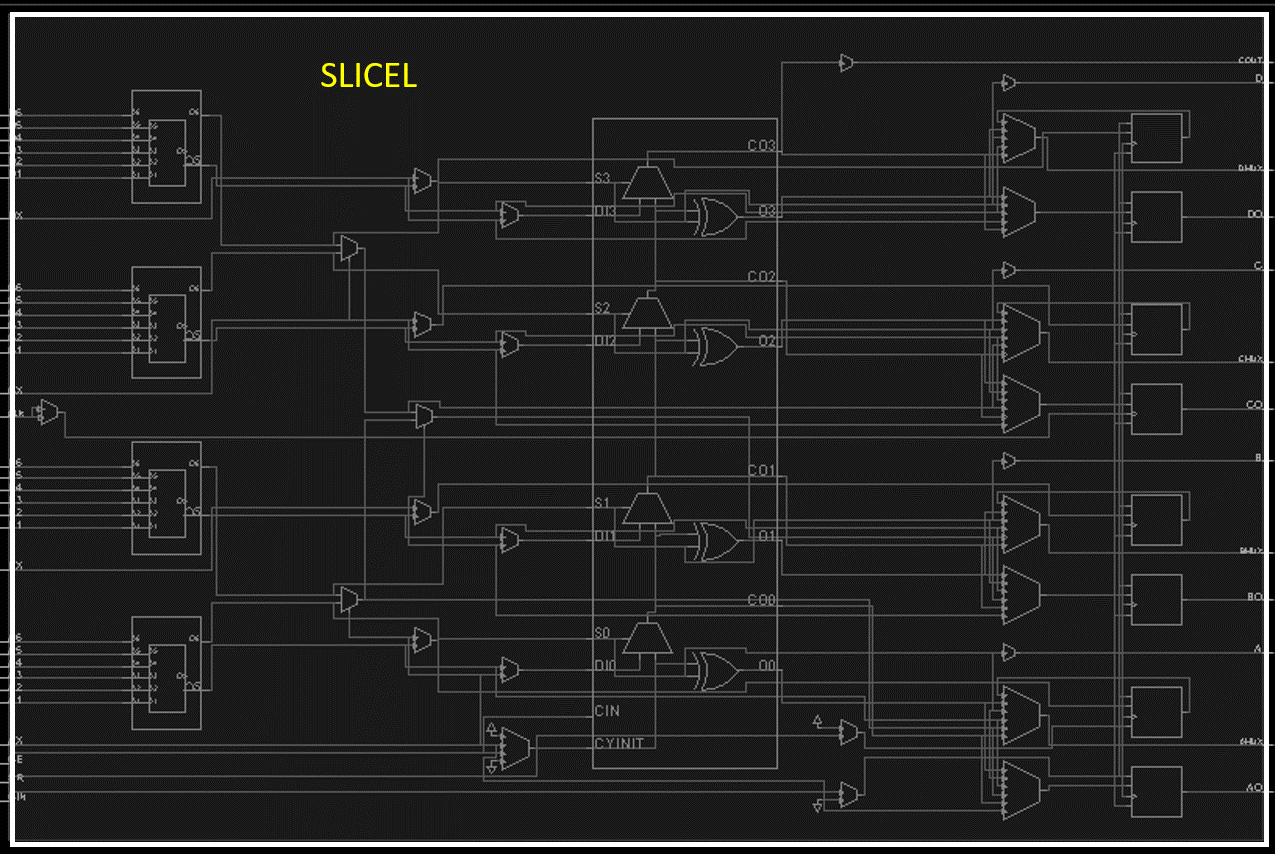
\includegraphics[width=1\linewidth]{site}
   \caption{}
   \label{fig:site1} 
\end{subfigure}

\begin{subfigure}[b!]{0.65\textwidth}
   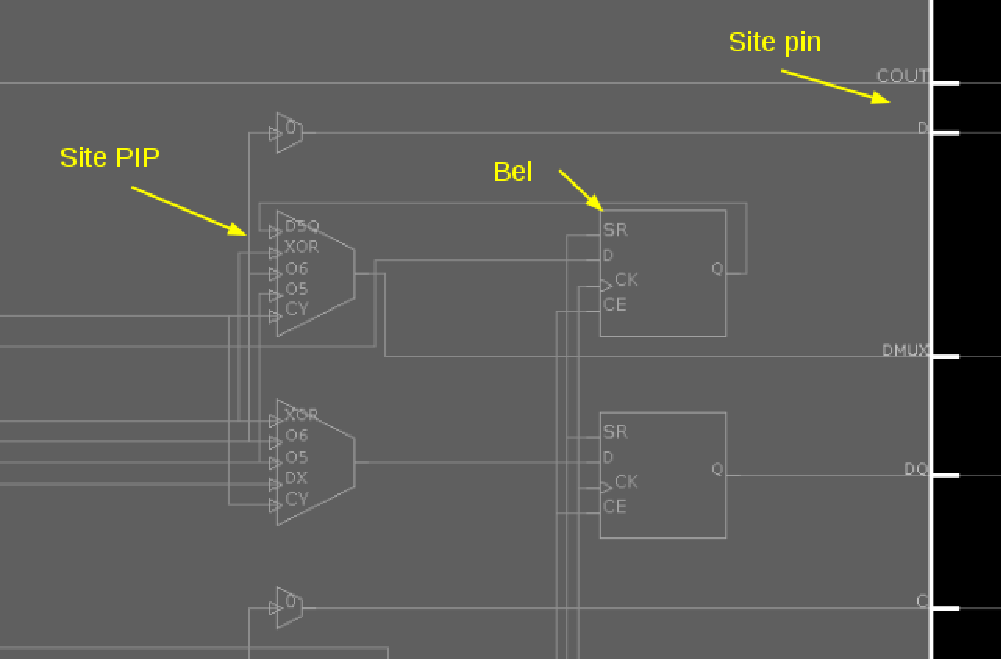
\includegraphics[width=1\linewidth]{subsite}
   \caption{}
   \label{fig:site2}
\end{subfigure}

\caption{(a) A highlighted example of a SLICEL \cls{Site} in a CLBLL \cls{Tile}
of an Artix7 FPGA. (b) The basic components of a \cls{Site} in a
Xilinx FPGA.}
\label{fig:site}
\end{figure}

Each \cls{Tile} can contain one or more \cls{Primitive Site}s (often shortened
to \cls{Site}). As \autoref{fig:tileExample} shows, CLBLL \cls{Tile}s
have two \cls{Site}s, INT\_L \cls{Tile}s have one \cls{Site}, and VBRK \cls{Tile}s
have none. A \cls{Site} is the part within a \cls{Tile} that actually performs
its ``useful'' function. The remainder of the \cls{Tile} is used to wire signals
to/from its \cls{Site}s. \autoref{fig:site} shows a SLICEL, one of the
\cls{Site}s within a CLBLL \cls{Tile}. As the figure shows, there are three main
components to \cls{Site}s in Xilinx FPGAs:

\begin{itemize}
  \item \cls{Site} \cls{PIP}s: Reconfigurable routing PIPs used for intrasite
  routing (also called routing muxes). In Vivado, \cls{Site} \cls{PIP}s are usually configured
  automatically as cells in a design are being placed (based on cell properties
  and placement location).
  \item \cls{BEL}s: \pgm{B}asic \pgm{EL}ements are hardware components within
  the \cls{Site} for implementing digital logic. For example, LUT \cls{BEL}s within a SLICEL
  are used to implement logic equations, and Flip Flop \cls{BEL}s are used
  as storage. In a synthesized netlist, design elements are mapped to physical
  \cls{BEL}s during implementation.
  \item \cls{Site Pin}s: \cls{Site} input and output. These pins are connected
  to \cls{Wire}s of the parent \cls{Tile} and typically drive general
  fabric.
\end{itemize}

\subsubsection{Wires and PIPs} \label{wireSection}
 
FPGA components are connected together using metal \cls{Wire}s (called
\cls{Node}s in Vivado). In order to make the FPGA reconfigurable,
\cls{Wire}s are connected together through Programmable Interconnect Points
(\cls{PIP}s). Individual \cls{PIP}s can be enabled or disabled as a design is
being routed, and a string of enabled \cls{PIP}s uniquely identify the
used \cls{Wire}s of a physical route. \cls{PIP}s are most commonly
found in Switchbox \cls{Tile}s, and enable a single wire to be routed to many
different locations in the FPGA. \autoref{fig:switchboxPIP} shows an
example of a switchbox.

\begin{figure}[H]
	\centering
	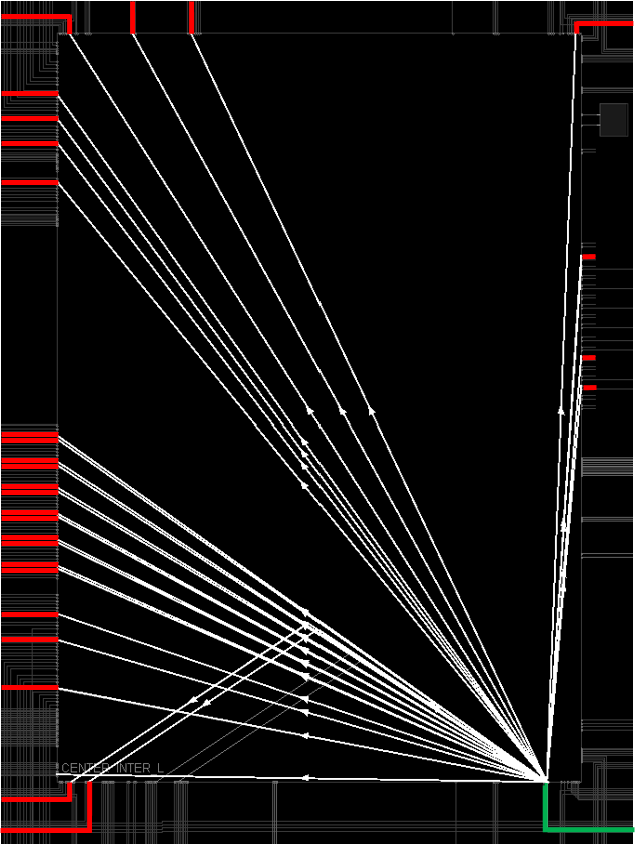
\includegraphics[width=0.45\columnwidth]{pipExample}
	\caption{An example of PIP wire connections in a device. The green wire
	represents the source wire, and the red wires represent all possible sink
	wires in the Switchbox. The highlighed white sections of the figure are PIP
	connections.}
	\label{fig:switchboxPIP}
\end{figure} 
 
\subsection{Device Data Structures} \label{devicesRS2}
In the original RapidSmith, the \cls{Device} architecture stopped at the
\cls{Site} level. A \cls{Site} was considered a black box who could be
configured using string attributes, but the actual components were unknown.
RS2 extends the \cls{Device} architecture to include all components
\pgm{within} a \cls{Site} as well. \autoref{fig:deviceDataStructures}
shows the new device data structure hierarchy, which can be found in the {\em
edu.byu.ece.rapidSmith.device} package.

\begin{figure}[H]
	\centering
	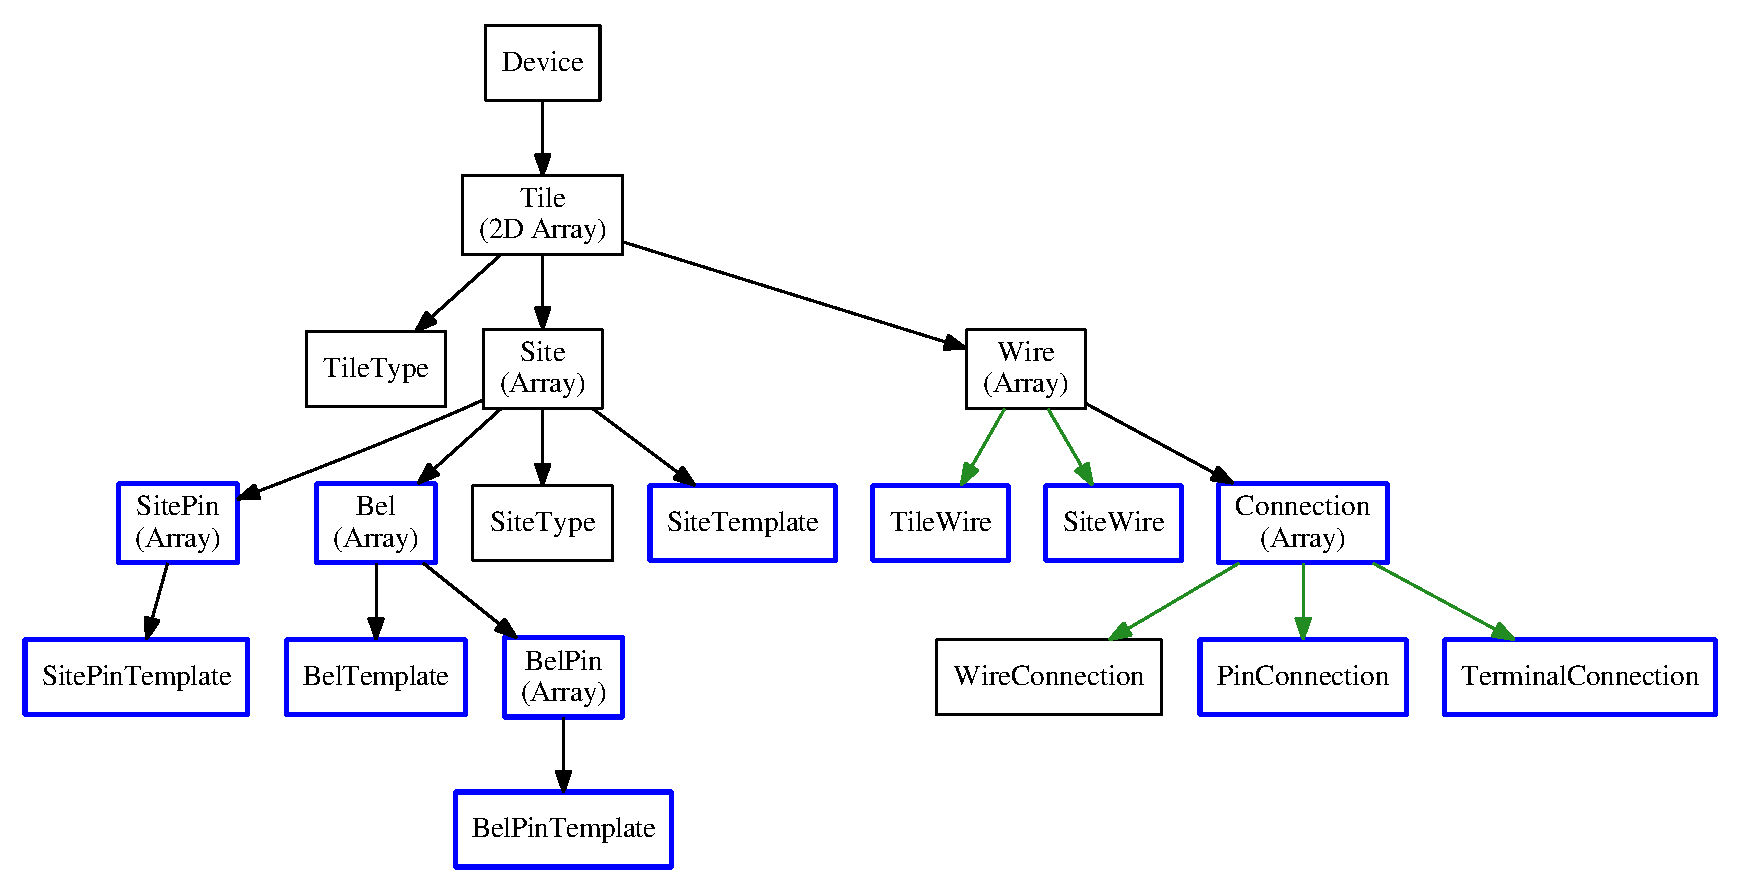
\includegraphics[width=1\columnwidth]{deviceDS.eps}
	\caption{RS2 \cls{Device} data structure tree. Green arrows represent
	inheritance, and black arrows represent association. Classes and Interfaces
	bolded in blue are new to RS2.}
	\label{fig:deviceDataStructures}
\end{figure}

\noindent
The classes and interfaces within {\em edu.byu.ece.rapidSmith.device} are named
to reflect the terminology used by Xilinx. Many classes that exist in Vivado's
Tcl interface have a direct map to a class in RS2 (such as a \cls{Tile}).
Because of this, most RS2 data structures represent a straightforward
part of a Xilinx FPGA, The reader is referred to the documentation in the
source code to learn more about each data structure. Also, The
\pgm{DeviceBrowser} and \pgm{DeviceAnalyzer} programs described in 
\autoref{examples} illustrate how to load and browse a device down to the
\cls{Tile} and \cls{Site} levels.

\subsubsection{Templates}
As \autoref{fig:deviceDataStructures} shows, there are several template
classes in RS2. Template classes are used to specify the configuration of
certain structures only once, and then reuse the configuration across
identical objects. The usefulness of templates is best shown with an example. In
an Artix-7 {\em xc7a100tcsg324} part, there are 11,100 \cls{Site}s of type
SLICEL. Each of these SLICELs have 215 \cls{BEL}s, \cls{Site} \cls{Pin}s, and
\cls{Site} \cls{PIP}s combined. In order to save memory, RS2
lazily creates these objects only when a SLICEL \cls{Site} is being used. The
alternative would be to create each of the objects when a device is loaded.
Template classes should \pgm{NOT} be used by the normal user. When creating
algorithms using RS2's API, use the non-template version of classes.

\subsubsection{WireEnumerator} \label{wireEnum}
Wires with the same name can occur several times throughout a Xilinx FPGA
device. For example, the wire ``CLBLL\-\_L\_C2'' exists in every \cls{Tile} of
type ``CLBLL\_L''. In order to make the device files small, each uniquely named \cls{Wire}
is assigned an integer enumeration. This avoids moving strings around in
memory which would be costly in terms of both space and comparison times.
RS2 manages all uniquely named wires in an FPGA family with a
\cls{WireEnumerator}. The \cls{WireEnumerator} class has methods that convert to
and from the wire name and enumeration of a \cls{Wire}, and also stores other
\cls{Wire} information such as direction and type. In previous versions of
RapidSmith, the user had to use the \cls{WireEnumerator} extensively while
building CAD tools. RS2 has changed this, largely abstracting the
\cls{WireEnumerator} away in favor of more convenient methods in all classes and
interfaces that deal with \cls{Wire}s. For example, the name or enumeration of a
\cls{Wire} can now be obtained with the function calls {\em Wire.getWireName()}
and {\em Wire.getWireEnum()} respectively. A handle to the
\cls{WireEnumerator} still exists in the \cls{Device} class for those who
want to use it, but this is not recommended. 

\subsubsection{TileWire and SiteWire} \label{wires}
\cls{Wire}s in RS2 are uniquely identified not only by their name
(or enumeration), but also by the \cls{Tile} or \cls{Site} in which they exist.
RS2 introduces the \cls{TileWire} and \cls{SiteWire} classes to
encapsulate this information for the user. Many functions in RS2 now
return a \cls{TileWire} or \cls{SiteWire} (wrapped in a generic \cls{Wire}
object) to the user instead of an integer wire enumeration.

\subsubsection{Wire and Connection Interfaces}
As \autoref{fig:deviceDataStructures} shows, there are two classes that
inherit the \cls{Wire} interface (described in \autoref{wires}) and
three classes that inherit the \cls{Connection} interface (described in 
\autoref{otherConns}). In general, most methods in RS2 return the
generic interface instead of the subclasses. When creating CAD tools in
RS2, it is suggested that the user use these interfaces. Several of the
examples referenced in \autoref{examples} demonstrate the use of these
interfaces.

\subsection{Loading a Device} \label{sec:loadingDevice}

The code sample below demonstrates how to load a supported device in
RS2.

\begin{lstlisting}[caption=Loading a Device, label=code:loadDevice]
Device device = RSEnvironment.defaultEnv().getDevice("xc7a100tcsg324");
//or
Device deviceReloaded = RSEnvironment.defaultEnv().getDevice("xc7a100tcsg324", true);
\end{lstlisting}

\noindent The first function call will only load the device into memory if it
has not yet been loaded. If it has been loaded, then the cached \texttt{Device}
data structure will be returned. The second function call will reload the device from
disk, creating a completely separate \texttt{Device} data structure. This is
useful when implementing multi-threaded code that targets the same part.
\textbf{NOTE:} When a Vivado design is loaded into RS2 via a RSCP, the
corresponding device is also loaded.

\subsection{Supported Device Files} \label{sec:supportedDevices}
RS2 currently supports the following device families and parts.

\begin {itemize}
  \item Artix7 
  	\begin{itemize}
  	  \item xc7a100t-csg324-3
  	\end{itemize}
  \item Kintex Ultrascale (kintexu)
    \begin{itemize}
  	  \item xcku025-ffva1156 
  	\end{itemize}
\end{itemize}

\noindent Section \ref{sec:installingDeviceFiles} describes how to install new
RS2 device files if you wish to add to this list. 
